\documentclass[openany]{ntuthesis}

\usepackage{times}
\usepackage{verbatim}
\usepackage{color}
\usepackage{url}
\usepackage{graphicx}
\usepackage{array}
\usepackage{hyperref}


% Using the tex-text mapping for ligatures etc.
\defaultfontfeatures{Mapping=tex-text}

% Set the default fonts
\setmainfont{Times New Roman}
\setCJKmainfont{BiauKai}

% Your information goes here
%%% Use packages.
\usepackage{color}
%\usepackage{enumitem} % will cause error in TVCG template
%\usepackage{amsmath} % already inlucded in EG template
%\usepackage{amssymb} % already inlucded in EG template
% \usepackage{algorithm}
%\usepackage{algorithmic}
% \usepackage{algpseudocode}
%\renewcommand{\algorithmicrequire}{\textbf{Input:}}  % Use Input in the format of Algorithm
%\renewcommand{\algorithmicensure}{\textbf{Output:}} % Use Output in the format of Algorithm
%\usepackage{booktabs}
\usepackage{graphicx}
\usepackage{ulem}
\usepackage{ifthen}

\newcommand{\projectName}{Nail+}

\normalem

%%% The color definition.
\definecolor{gray}{rgb}{0.5,0.5,0.5} 
\definecolor{green}{rgb}{0, 0.4, 0}
\definecolor{orange}{rgb}{1, 0.5, 0}
\definecolor{mahogany}{rgb}{0.75, 0.25, 0.0}
\definecolor{purple}{rgb}{0.6, 0, 0.6}
\definecolor{purple}{rgb}{0.6, 0, 0.6}
\definecolor{darkgreen}{rgb}{0, 0.4, 0} 
\definecolor{frenchblue}{rgb}{0.0, 0.45, 0.73}

%%% Editing comments.
% ignore this
\newcommand{\ignore}[1]{}
% comment
\newcommand{\cmt}[1]{\begin{sloppypar}\large\textcolor{red}{#1}\end{sloppypar}}
% the note in the paper
\newcommand{\note}[1]{\cmt{Note: #1}}
%\newcommand{\todo}[1]{ \textcolor{red}{[{\bf TODO}: #1]}}
% the part to revise
\newcommand{\torevise}[1]{ \textcolor{red}{#1}}
% text copied from somewhere
\newcommand{\copied}[1]{ \textcolor{red}{[COPIED: #1]}}
% the old version
\newcommand{\old}[1]{ \textcolor{gray}{#1}}
\usepackage{color}


%%% Frequently used terms.
\newcommand{\etal}{\textit{et~al.}~}    % disabled because defined elsewhere
\newcommand{\ie}{\textit{i.e.},~}
\newcommand{\eg}{\textit{e.g.},~}
\newcommand{\figname}{Figure}
\newcommand{\tabname}{Table}
\newcommand{\secname}{Section}
\newcommand{\algoname}{Algorithm}
\newcommand{\eqname}{Eq.}

%%% Personal editing recognition.
\newboolean{revising}
\setboolean{revising}{false}
\ifthenelse{\boolean{revising}}
{
    \newcommand{\add}[1]{\textcolor{darkgreen}{#1}}
%    \newcommand{\delete}[1]{\sout{#1}}
    \newcommand{\delete}[1]{}
    \newcommand{\remove}[1]{\delete{#1}}
    \newcommand{\mike}[1]{\textcolor{orange}{#1}}
    \newcommand{\mikeignore}[1]{\sout{#1}}
    \newcommand{\yiling}[1]{\textcolor{frenchblue}{#1}}
    \newcommand{\yilingreplace}[2]{{\sout{#1}} \textcolor{frenchblue}{#2}}
    \newcommand{\liwei}[1]{\textcolor{purple}{#1}}
    \newcommand{\liweiignore}[1]{\sout{#1}}
    \newcommand{\liweireplace}[2]{{\sout{#1}} \textcolor{purple}{#2}} 
    \newcommand{\dayuan}[1]{\textcolor{frenchblue}{#1}}
    \newcommand{\dayuanreplace}[2]{{\sout{#1}} \textcolor{frenchblue}{#2}}
    \newcommand{\jesse}[1]{\textcolor{orange}{#1}}
    \newcommand{\jessereplace}[2]{{\sout{#1}} \textcolor{orange}{#2}}
    \newcommand{\kp}[1]{\textcolor{blue}{#1}}
    \newcommand{\kpreplace}[2]{{\sout{#1}} \textcolor{blue}{#2}}
    \newcommand{\steven}[1]{\textcolor{purple}{#1}}
    \newcommand{\stevenreplace}[2]{{\sout{#1}}
    \textcolor{purple}{#2}}
} {
    \newcommand{\add}[1]{#1}
    \newcommand{\delete}[1]{}
    \newcommand{\remove}[1]{}
    \newcommand{\replace}[2]{#2}
    \newcommand{\mike}[1]{#1}
    \newcommand{\mikeignore}[1]{}
    \newcommand{\yiling}[1]{#1}
    \newcommand{\yilingreplace}[2]{#2}
    \newcommand{\liwei}[1]{#1}
    \newcommand{\liweireplace}[2]{#2}
    \newcommand{\dayuan}[1]{#1}
    \newcommand{\dayuanreplace}[2]{#2}
    \newcommand{\jesse}[1]{#1}
    \newcommand{\jessereplace}[2]{#2}
    \newcommand{\kp}[1]{#1}
    \newcommand{\kpreplace}[2]{#2}
    \newcommand{\steven}[1]{#1}
    \newcommand{\stevenreplace}[2]{#2}
}
% author: Tz-Huan Huang [http://www.csie.ntu.edu.tw/~tzhuan]

% ----------------------------------------------------------------------------
% "THE CHOCOLATE-WARE LICENSE":
% Tz-Huan Huang wrote this file. As long as you retain this notice you
% can do whatever you want with this stuff. If we meet some day, and you think
% this stuff is worth it, you can buy me a chocolate in return Tz-Huan Huang
% ----------------------------------------------------------------------------

% Syntax: \var{English}{Chinese}
\university{National Taiwan University}{國立臺灣大學}
\collage{College of Electrical Engineering and Computer Science}{電機資訊學院}
\institute{Department of Computer Science and Information Engineering}{資訊工程學系}
\title{A Comparison of Soft Keyboards on Circular Smartwatches}{智能手錶上的虛擬鍵盤之比較}
\author{Reinhard Pointner}{郝瑞尼}
\studentid{R02922148}
\advisor{Mike Y. Chen, Ph.D.}{陳彥仰 博士}
\year{2017}{106}
\month{July}{7}
\day{19}


\begin{document}

\frontmatter

\makecover

\makecertification

%\begin{acknowledgementszh}
%\end{acknowledgementszh}

%\begin{acknowledgementsen}
% TODO
%\end{acknowledgementsen}

%\begin{abstractzh}
% TODO 中文摘要
% \end{abstractzh}


\begin{abstracten}
% 1. Current Situation
% 2. Problem Statement
% 3. Proposed Solution
% 4. Solution Details
% 5. Results and Contributions

Smartwatches, wearable electronics, and other miniature devices are becoming increasingly popular. However, text input on such small devices remains a challenge due to small form factors, especially for non-Latin languages that require more complex key entry techniques. We implement and compare 3 fully functional soft keyboards for typing Mandarin Chinese using the Hanyu Pinyin system on the latest generation of circular smartwatch devices. We introduce 2 such novel adaptive keyboards called Growing Finals and Pinyin Syllables,  which change dynamically based on the current input and the limited number of possible subsequent letters, optimize available screen size, and improve better user experience on small screens.
Our evaluation is based on a user study with 15 participants and shows input speeds of around 19.4 CCPM for Growing Finals and 18.5 CCPM for Pinyin Syllables after 20 minutes of practice. More than half of the participants preferred one of these input methods over the standard QWERTY keyboard.
% We discovered from participants' keyboard activites that over half preferred one of our proposed novel input methods versus standard QWERTY input due to lesser frustration and fewer error encounters. 
\end{abstracten}


\begin{comment}
\category{H.5.2.}{Information Interfaces and Presentation (e.g. HCI)}{User Interfaces; Input devices and strategies (e.g., mouse, touchscreen)}

\terms{Text Entry, Pinyin, Smartwatch, Human Factors, Performance}

\keywords{Chinese text entry; smartwatch; adaptive keyboard}
\end{comment}


\tableofcontents
\listoffigures
% \listoftables

\mainmatter

% Your thesis goes here
\chapter{Introduction}
\label{c:intro}


% Unlike western languages such as English, which utilize keybaord devices that map directly to the letters of their words, Chinese characters consist of at least tens of thousands of characters that cannot be trivially mapped into computing keyboard devices. One form of input that hardware designers have chosen is to alternatively capture existing Latin-based romanization systems that can rely on existing computing keyboard devices to similarly type Chinese characters. Such mechanisms have greatly enabled many users of native Chinese language users to perform many computing tasks analogously to their western counterparts ranging from typing documents, browsing the web, and communicate with others in social media, which eventually led to the Chinese language being one of the most popular languages utilized on the internet.

As miniaturization and battery technology improve, major electronics manufacturers have created smartwatches, which contain the processing power and memory of a computer or a smartphone and feature 4G connectivity, GPS, accelerometers, heart beat sensors and so on. These smartwatches can provide interactions with the digital world without one having to carry a phone, for example when doing outdoor sports.

Even though smartwatch devices have become more and more comparable to smartphones in terms of computing power, user interaction can be tricky due to the limited screen size and small form factor. Voice input, while reliable and fast in most cases, is not always socially acceptable and may not be a viable option in noisy environments or when entering out-of-vocabulary text such as addresses or passwords. As such, easy-to-use and accurate text input methods are an important aspect of smartwatch devices, and platform developers such as Google now include touch-based text input methods by default and allow users to add 3rd party input methods.

% ONE SUGGESTION: possibly mention that existing input techniques that still assume conventional QWERTY keyboard assumptions do not consider the smaller form factors and constrained screen sizes found in the newer contributions and growing ubiquity of smartwatches (e.g., not optimize, come up with something more appropriate)

In this paper, we design and implement 3 fully functional Chinese soft keyboards for modern circular smartwatches. We propose an adaptive quasi-QWERTY keyboard that enlarges the next possible keys to improve speed and accuracy, an adaptive 2-stage keyboard that allows any Pinyin syllable to be entered with a fixed number of 2 key presses, and a standard QWERTY keyboard with 26 keys optimized for the small screen size. All 3 keyboard implementations use the same Pinyin-to-Chinese-Character conversion engine to allow for a fair comparison in our user study.

\begin{figure}
  \centering
  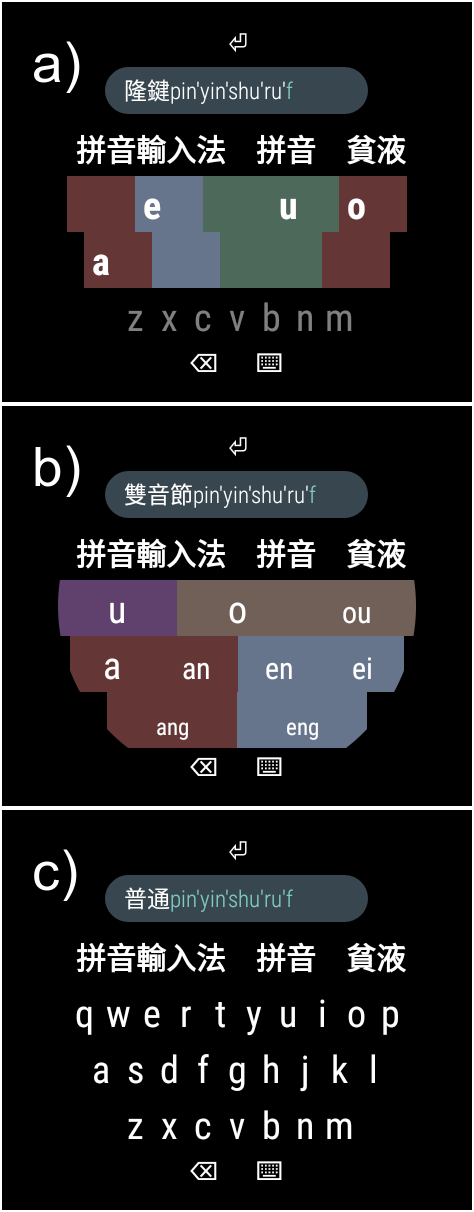
\includegraphics[width=\textwidth,height=0.9\textheight,keepaspectratio]{figures/stripe_banner_layouts}
  \caption{Keyboards for Chinese text input on smartwatches used in our study: (a) Growing Finals, (b) Pinyin Syllables and (c) Standard QWERTY.}~\label{fig:figure1}
\end{figure}

\chapter{Related Work}
\label{c:related}


% direct references
% 1. small screen text-entry
% 2. feature phone text-entry
% 3. menu- or gesture-driven text-entry

% peripheral references
% 1. handwriting or gesture modalitiy
%    - forgetfulness
%    - writing is slow
%    - difficult for small form factors
% 2. voice modality
%    - uncomfortable in quiet environments
%    - unreliable in loud environments
%    - becomes complicated in certain Chinese language context

Text entry on small touch screen devices is a well explored topic \cite{Chen:2014:STE:2642918.2647354}\cite{Oney:2013:ZDQ:2470654.2481387}\cite{Shao:2016:SSK:2935334.2935336}\cite{Yi:2017:CRK:3025453.3025454}, but input methods for more complex writing systems with more than 26 Latin characters \cite{Lunde:2008:CIP:1525605} such as Chinese used by more than 1 billion native speakers are rarely studied.

Before the advent and widespread use of touchscreen phones, Liu et al have compared the performance of handwriting recognition (15 CCPM), a standard QWERTY keyboard (14 CCPM) and a static 2-stage consonant + vowel keyboard (9 CCPM) \cite{Liu:2009:IUP:1613858.1613928} for Chinese character input on a PDA with a stylus and explored Chinese text entry using a rotary input with RotaTxt (6 CCPM) \cite{Liu:2008:RCP:1409240.1409265}. The low input speed of these early works can partially be explained by the lack of smart Pinyin-to-Chinese-Character conversion engines that could run on the limited hardware of the time.

More recently, inspired by ShapeWriter \cite{Zhai:2003:SWS:642611.642630}, Liu et al \cite{Liu:2012:PPM:2371574.2371614} improve upon the standard QWERTY keyboard for Chinese input on smartphones by adding a pie menu to each initial key to allow users to write a complete Pinyin syllable with one key press directly followed by multiple swipe motions to select the final letter sequence from the pie menu before lifting the finger to commit the Pinyin syllable closing the pie menu. Unfortunately, the prototype only achieved 25 CCPM with the pie menu augmented keyboard compared to 30 CCPM achieved with the standard QWERTY baseline.

\chapter{Three Pinyin Input Methods}
\label{c:prototypes}


We have designed and implemented 3 Chinese keyboards for circular smartwatches. Figure \ref{fig:figure1} shows our three prototypes. Each prototype has been implemented natively for Android Wear 2.0 and tested on an LG Watch Style. This smartwatch has a round 1.2" (30 mm) screen. Our implementation is open-source software, so that other researchers or developers can reuse and build upon our code.\footnote{https://github.com/rednoah/android-wear-pinyin}




\section{Growing Finals}
The Growing Finals keyboard (Figure \ref{fig:figure1}a) exploits an intrinsic characteristic of the Pinyin romanization system: out the 26 letters of the Latin alphabet, 23 can appear as the first letter in a Pinyin syllable, while the remaining 0 to 4 Latin letters of any Pinyin syllable are composed from only 9 unique Latin characters. Liu, et al. have previously exploited this characteristic in PinyinPie \cite{Liu:2012:PPM:2371574.2371614}.
Further research revealed that after selecting the first letter from a list of 23 options is entered, entering the remaining letters of any Pinyin syllable requires no more than 6 unique possible next letters (including the syllable separator \' if necessary) in any input state.
Hence, the Growing Finals keyboard will present a full QWERTY keyboard in its initial state and the---depending on the input---adapt and enlarge possible next letters while preserving the general QWERTY layout (Figure \ref{fig:figure2}). This allows for significantly larger keys after entering the initial letter for each syllable and thus improved input speed and accuracy according to Fitts' law.





\begin{figure}
  \centering
  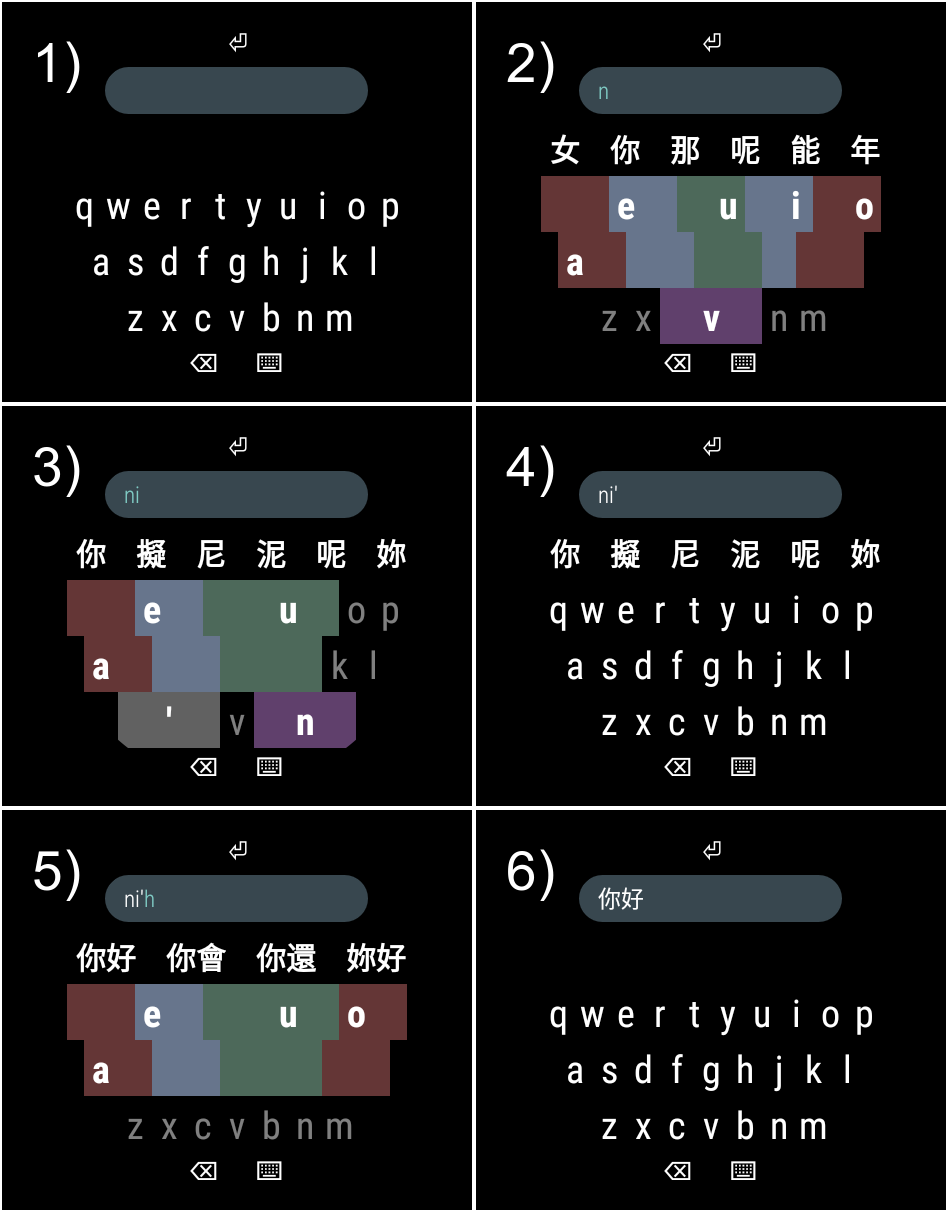
\includegraphics[width=1\columnwidth]{figures/sequence_GrowingFinals}
  \caption{Input sequence for the word 你好 (Pinyin: nǐ hǎo) using Growing Finals: 1) Press n 2) Press i 3) Press ‘詞 4) Press h 5) Select 你好}~\label{fig:figure2}
\end{figure}






\section{Pinyin Syllables}
Each Pinyin syllable can be seen as a combination of an initial sound and a final sound. Initials with similar sounds (e.g., b and p) tend to be combined with a similar set of final sounds (e.g., bang and pang) due to language characteristics. An analysis of the language model reveals that for each of the 26 initial sounds, there are between 2 and 24 (\textit{M} = 15.4, \textit{SD} = 5.6) possible final sounds (including no final sound for vowels such as a and e).
The Pinyin Syllables input method implements a 2-stage design based on Pinyin initials and finals which allows users to enter any Pinyin syllable with exactly 2 keystrokes. The first stage uses a pseudo-QWERTY keyboard layout to leverage existing familiarity with the standard QWERTY keyboard layout. The u, i, and v keys have been removed, and keys for sh, zh, and ch have been added so that each key on the initial keyboard corresponds to exactly one initial sound. Once an initial key has been entered, the keyboard will adapt and display all possible finals for the current input state (Figure \ref{fig:figure3}). Helping with visual search, finals with similar sounds are grouped by colour and placed near corresponding QWERTY keys if possible. Depending on the entered initial, the second stage may contain between 2 and 24 buttons allowing for significantly larger buttons in most cases with the added benefit that a single key press that completes the pinyin syllable may correspond to more than one Latin letter.





\begin{figure}
  \centering
  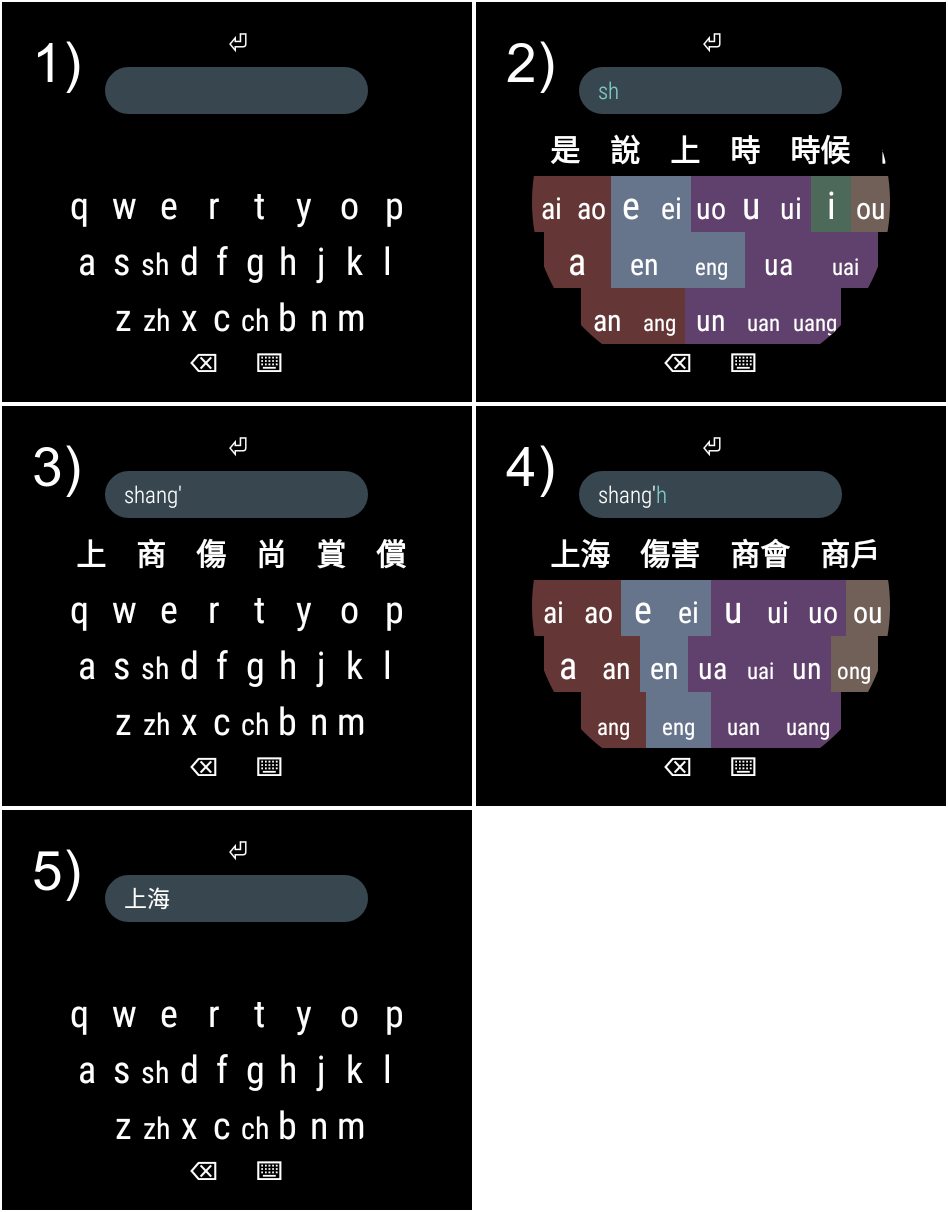
\includegraphics[width=1\columnwidth]{figures/sequence_PinyinSyllables}
  \caption{Input sequence for the word 上海 (pinyin: shàng hǎi) using Pinyin Syllables: 1) Press sh 2) Press ang 3) Press h 4) Select 上海}~\label{fig:figure3}
\end{figure}







\section{Standard QWERTY}
We implement the standard QWERTY keyboard with support for Chinese character entry (Figure \ref{fig:figure1}c) in addition to our two novel input methods to serve as a baseline for comparison. This keyboard design is used by almost all native speakers from China and language students from abroad that type Chinese characters on a computer and thus very familiar to most user.




\section{Common Features}
Each keyboard has a text field that shows the text that has been entered so far. Partial Pinyin input that defines the current state of the keyboard is highlighted. Selecting Chinese characters from the list of suggested candidates will replace the current Pinyin input with the selected Chinese characters and reset the keyboard to its original state for the next input sequence. The rotating hardware button can be used to scroll through the list of Chinese character suggestions without occluding the screen. The DELETE key can be used to delete the most recently entered Latin letter or Chinese character. Cursor movements are not supported.

We use the cross-platform native library RIME \cite{rime} as high-performance Pinyin-to-Chinese-Character conversion engine via Java Native Interface (JNI) on our Android Wear prototype. RIME uses state-of-the-art language models and algorithms with support for intelligent character level, phrase level and full sentence level Chinese character prediction based on complete or partial Pinyin sequences.

\chapter{Evaluation}
\label{c:evaluation}


The aim of this study is to understand the characteristics and user preferences for each of our three keyboard prototypes. We conducted a user study consisting of text-copy tasks using sentences sampled from the NUS SMS corpus compiled by Chen, et al. \cite{Chen2013} which consists of more than 30,000 Chinese short messages from Chinese users from all over China and is publicly available\footnote{https://github.com/kite1988/nus-sms-corpus}.
For our study, we only consider short messages from users living in Beijing who are known to speak the most standard dialect of Mandarin Chinese, in order to ensure that participants in our study are not confronted with unfamiliar local expressions or idioms. To focus only on Chinese sentences, we further restrict the study to samples that contain between 5 and 15 Chinese characters and no Latin letters or punctuation symbols.




\section{Participants}
We recruited 15 participants between the ages of 20 to 35 (\textit{M} = 25.9, \textit{SD} = 4.5) from various departments at our university and a nearby language training institution. 8 are native speakers of Chinese and 7 are highly proficient language students. 14 are right-handed and 1 is left-handed. All of them chose to wear the smartwatch on the wrist of their non-dominant hand and typed with the index finger of their dominant hand. 12 had never used a smartwatch before, the remaining 3 only for a short amount of time. All participants were very familiar with Chinese text entry using the standard QWERTY keyboard layout with the Pinyin system. Each participant was paid the equivalent of USD 5 in compensation for their time.





\section{Procedure}
Participants were seated in a quiet environment and were asked to rest their arm on the table in front of them to avoid fatigue. A computer screen in front of the participant instructed the participant which keyboard to use and what sentences to type. Figure \ref{fig:figure4} shows our user study setup. Participants were given a chance to experiment with each keyboard before starting the trials.







\begin{figure}
  \centering
  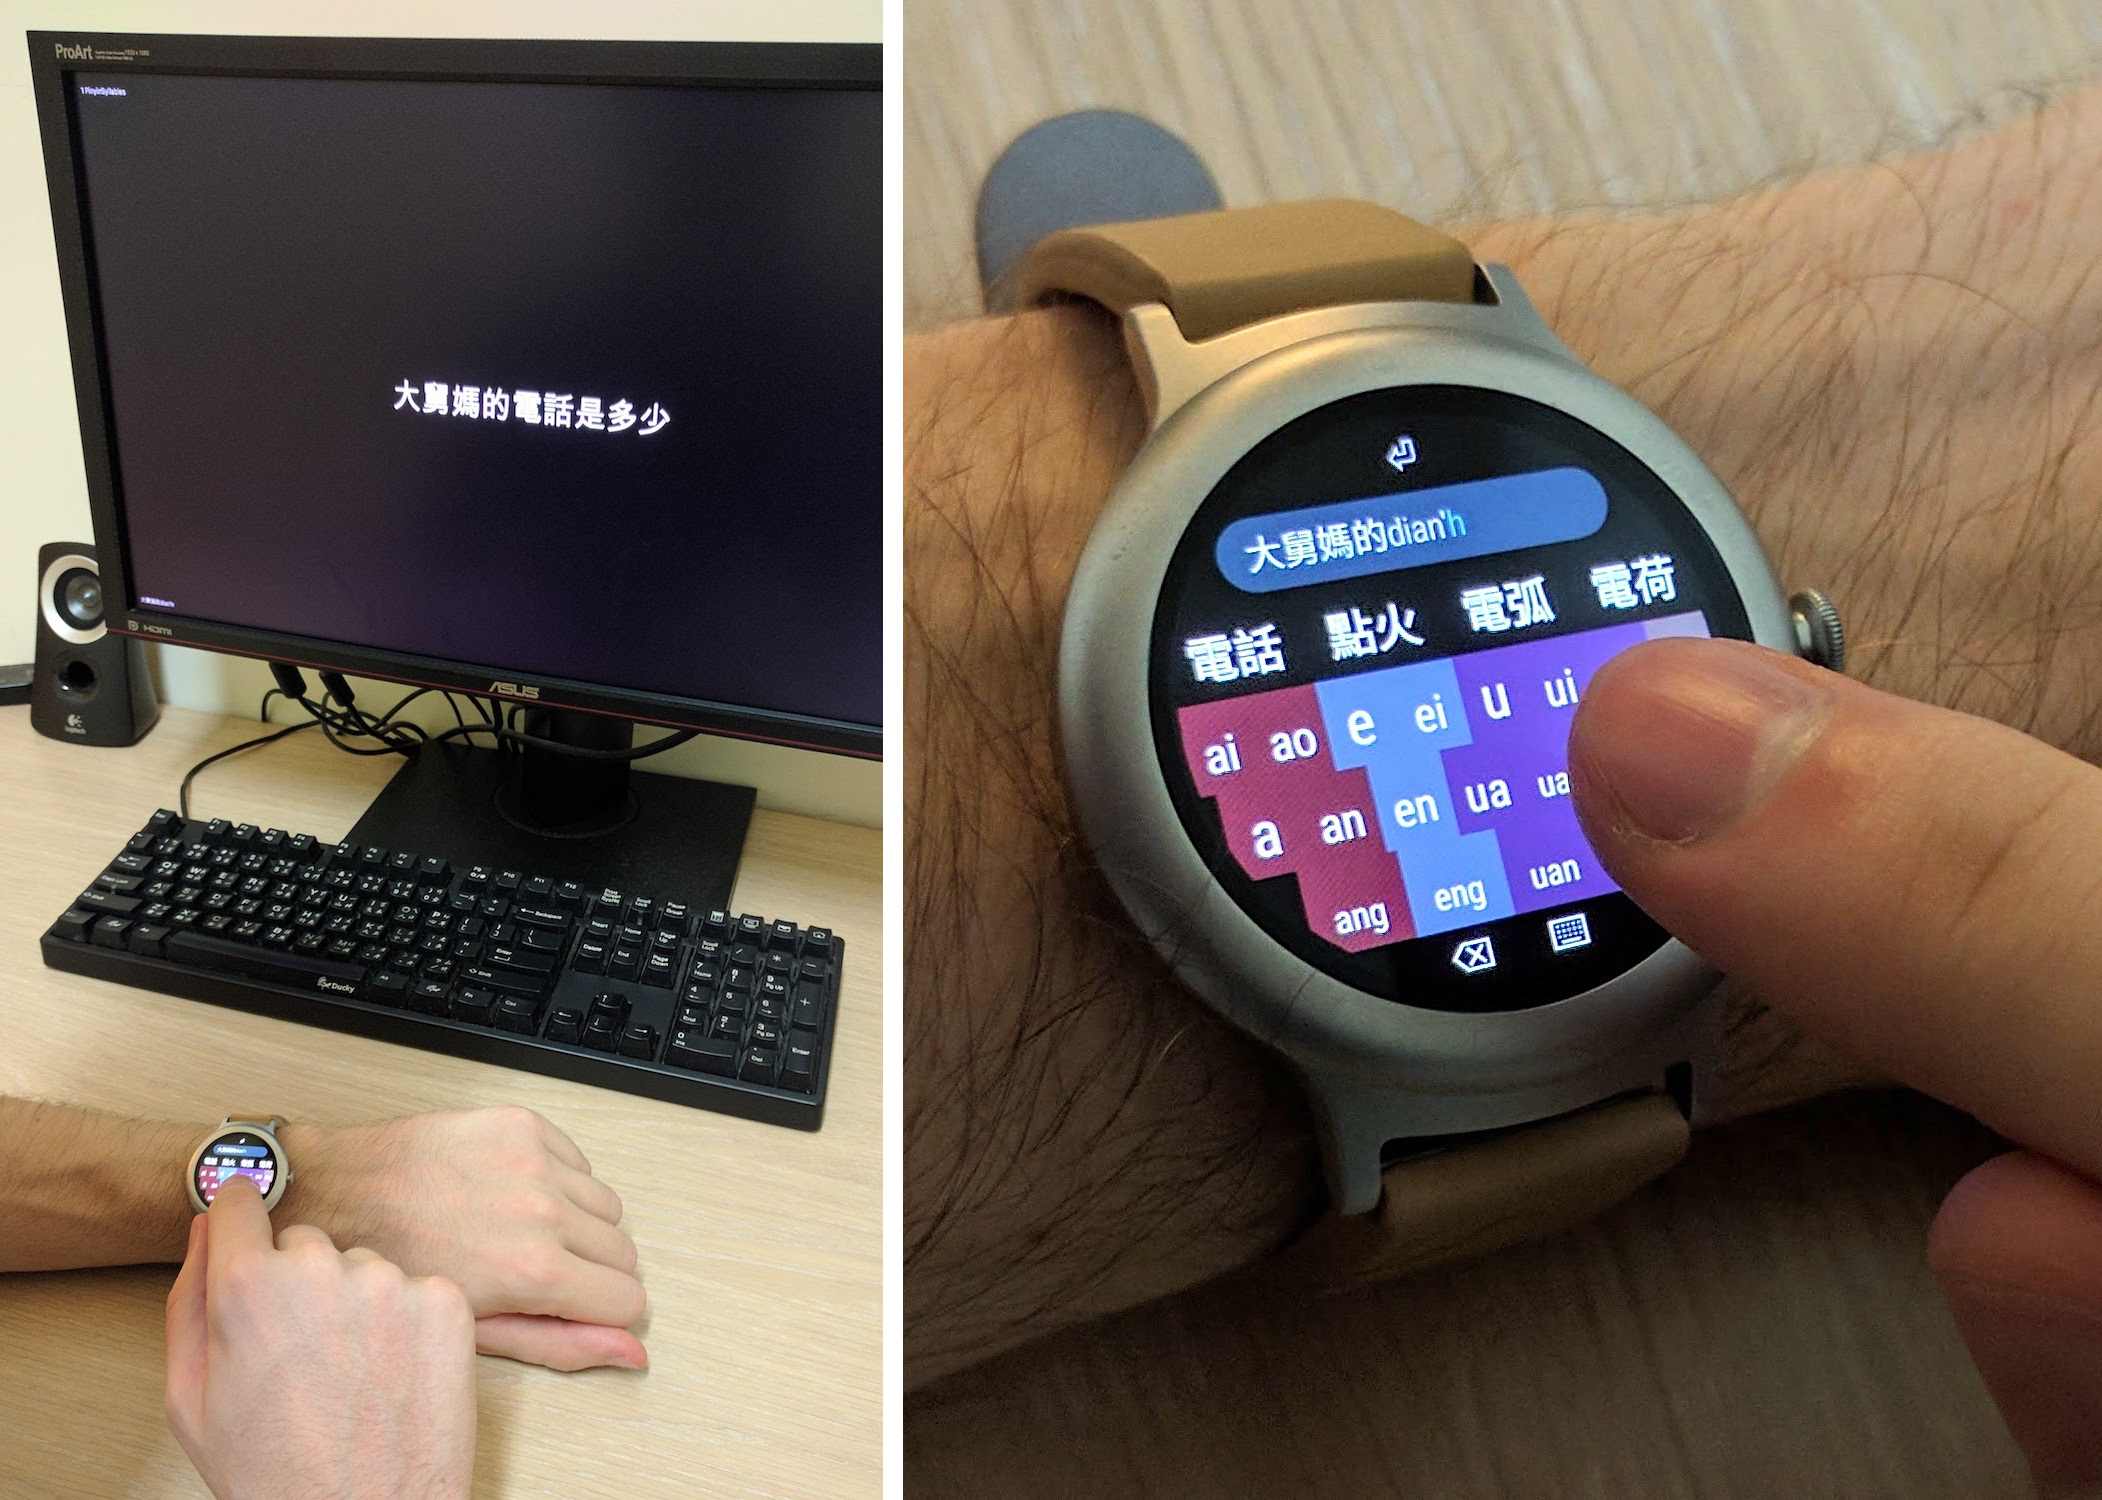
\includegraphics[width=1\columnwidth]{figures/user_study_setup}
  \caption{The setup of our user study.}~\label{fig:figure4}
\end{figure}








For each of the three keyboards, participants had to enter 25 sentences. The total of 3 $\times$ 25 = 75 sentences for all keyboard prototypes was randomly sampled from a specific subset of the NUS SMS corpus \cite{Chen2013} as explained above. These sentences contain only Chinese characters. All participants entered the same 75 sentences in the same order but the keyboard that was used for the first, second and third block of 25 sentences varied for each participant. We used Latin square design to counterbalance the order of keyboards.

Participants were asked to type as fast and as accurately as possible. For each sentence, before pressing the first key, participants were allowed to rest and memorize the sentence displayed on the computer screen in front of them for as long as they wanted. After entering each sentence, participants would press the ENTER key to continue to the next sentence.

After completing all trials, users were asked to rate each keyboard on a 5-point Likert scale and comment on positive and negative aspects of each keyboard.








\section{Results}
During the trials, we recorded 1,125 samples of sentence input representing close to 30,000 individual input events and 8.3 hours of non-stop typing data.


\begin{table}[]
\renewcommand{\arraystretch}{1.7}
\centering
\caption{Mean Chinese Characters per Minute (CCPM), Keystrokes per Chinese Character (KSPCC), Total Error Rate (TER) and Used Bandwidth (UBW) for each keyboard prototype. SDs are in parenthesis.}
\label{table:CCPM_KSPCC_TER_UBW}
\begin{tabular}{llll}

      & Growing Finals & Pinyin Syllables & QWERTY          \\ \hline
CCPM  & 19.39 (7.1)    & 18.51 (7.4)      & 22.39 (10.0)    \\
KSPCC & 3.72 (1.1)     & 2.98 (0.9)       & 3.79 (1.4)      \\
TER   & 7.72 (7.3)     & 9.49 (8.0)       & 12.21 (8.0)     \\
UBW   & 86.84 (11.8)   & 84.08 (12.2)     & 79.45 (12.6)    \\ \hline
\end{tabular}
\end{table}






\section{Text Entry Performance}
We measure text entry speed in Chinese characters per minute (CCPM) that we calculate as follows:

\[ CCPM = \frac{|C|}{T} \times 60 \]

where |\textit{C}| is the number of Chinese characters in the transcribed text and \textit{T} is the elapsed time in seconds from the first button press to the selection of the last Chinese character candidate before pressing ENTER.





In our study, the standard QWERTY keyboard slightly outperforms Growing Finals and Pinyin Syllables in terms of text entry speed (Table \ref{table:CCPM_KSPCC_TER_UBW}) with 22.4 CCPM (\textit{SD} = 10) but the high standard deviation indicates that it works better for some participants than others. Growing Finals offers the most stable input speed at 19.4 CCPM (\textit{SD} = 7) and Pinyin Syllables reached 18.5 CCPM (\textit{SD} = 7.5) on average despite steep learning curve.


\section{Error Rate}
We calculate the total error rate (TER) as described by Soukoreff et al \cite{Soukoreff:2003:MTE:642611.642632} that accounts for corrected and uncorrected errors. Considering the unique input characteristics of entering Chinese characters using Pinyin and candidate selections, we reinterpret the original formula for TER as follows:

\[ TER = \frac{E + D}{K + S + E + D} \]

where \textit{E} refers to the Levenshtein distance between the transcribed Chinese characters and the given sentence. \textit{D} refers to the number of DELETE events which may either delete the previously entered Latin Pinyin letter during Chinese character composition or a Chinese character after a Chinese character has been selected. \textit{K} and \textit{S} refer to key events for entering Latin Pinyin letters or selection events for converting Pinyin to Chinese characters respectively.


Due to the enlarged key size in many input states, Growing Finals and Pinyin Syllables have a lower TER of 7.7\% (\textit{SD} = 7.3) and 9.5\% (\textit{SD} = 8) respectively. Text entry on tiny QWERTY keyboards is feasible when carefully typing letter by letter but still error prone on small smartwatch devices \cite{Leiva:2015:TET:2702123.2702388}. The TER of 12.2\% (\textit{SD} = 8) reflects this fact.


\section{Keystrokes per Chinese Character}
Unlike Latin languages such as English, when entering Chinese characters using the Pinyin system, a single keystroke will not represent a single Chinese character entered, rather a sequence of keystrokes and candidate selections will eventually lead to one or more Chinese characters being entered. We compute keystroke per Chinese character (KSCC) as follows:
\[ KSPCC = \frac{K + S + D}{|C|} \]
where \textit{K}, \textit{S} and \textit{D} refer to key, selection or delete events and |\textit{C}| refers to the number of Chinese characters in the transcribed sentence.

Pinyin Syllables has the lowest and most stable KSCC at 3 (\textit{SD} = 0.9) because each pinyin syllable can be entered with a fixed number of 2 key press events, which means that higher input speeds can be expected once users fully memorize key locations and spend less time on visual search. The letter-by-letter input mechanics that Growing Finals and Standard QWERTY have in common leads to similar KSPCC values of 3.72 (\textit{SD} = 1.1) and 3.79 (\textit{SD} = 1.4) respectively.
 
 
 
 \begin{figure}
  \centering
  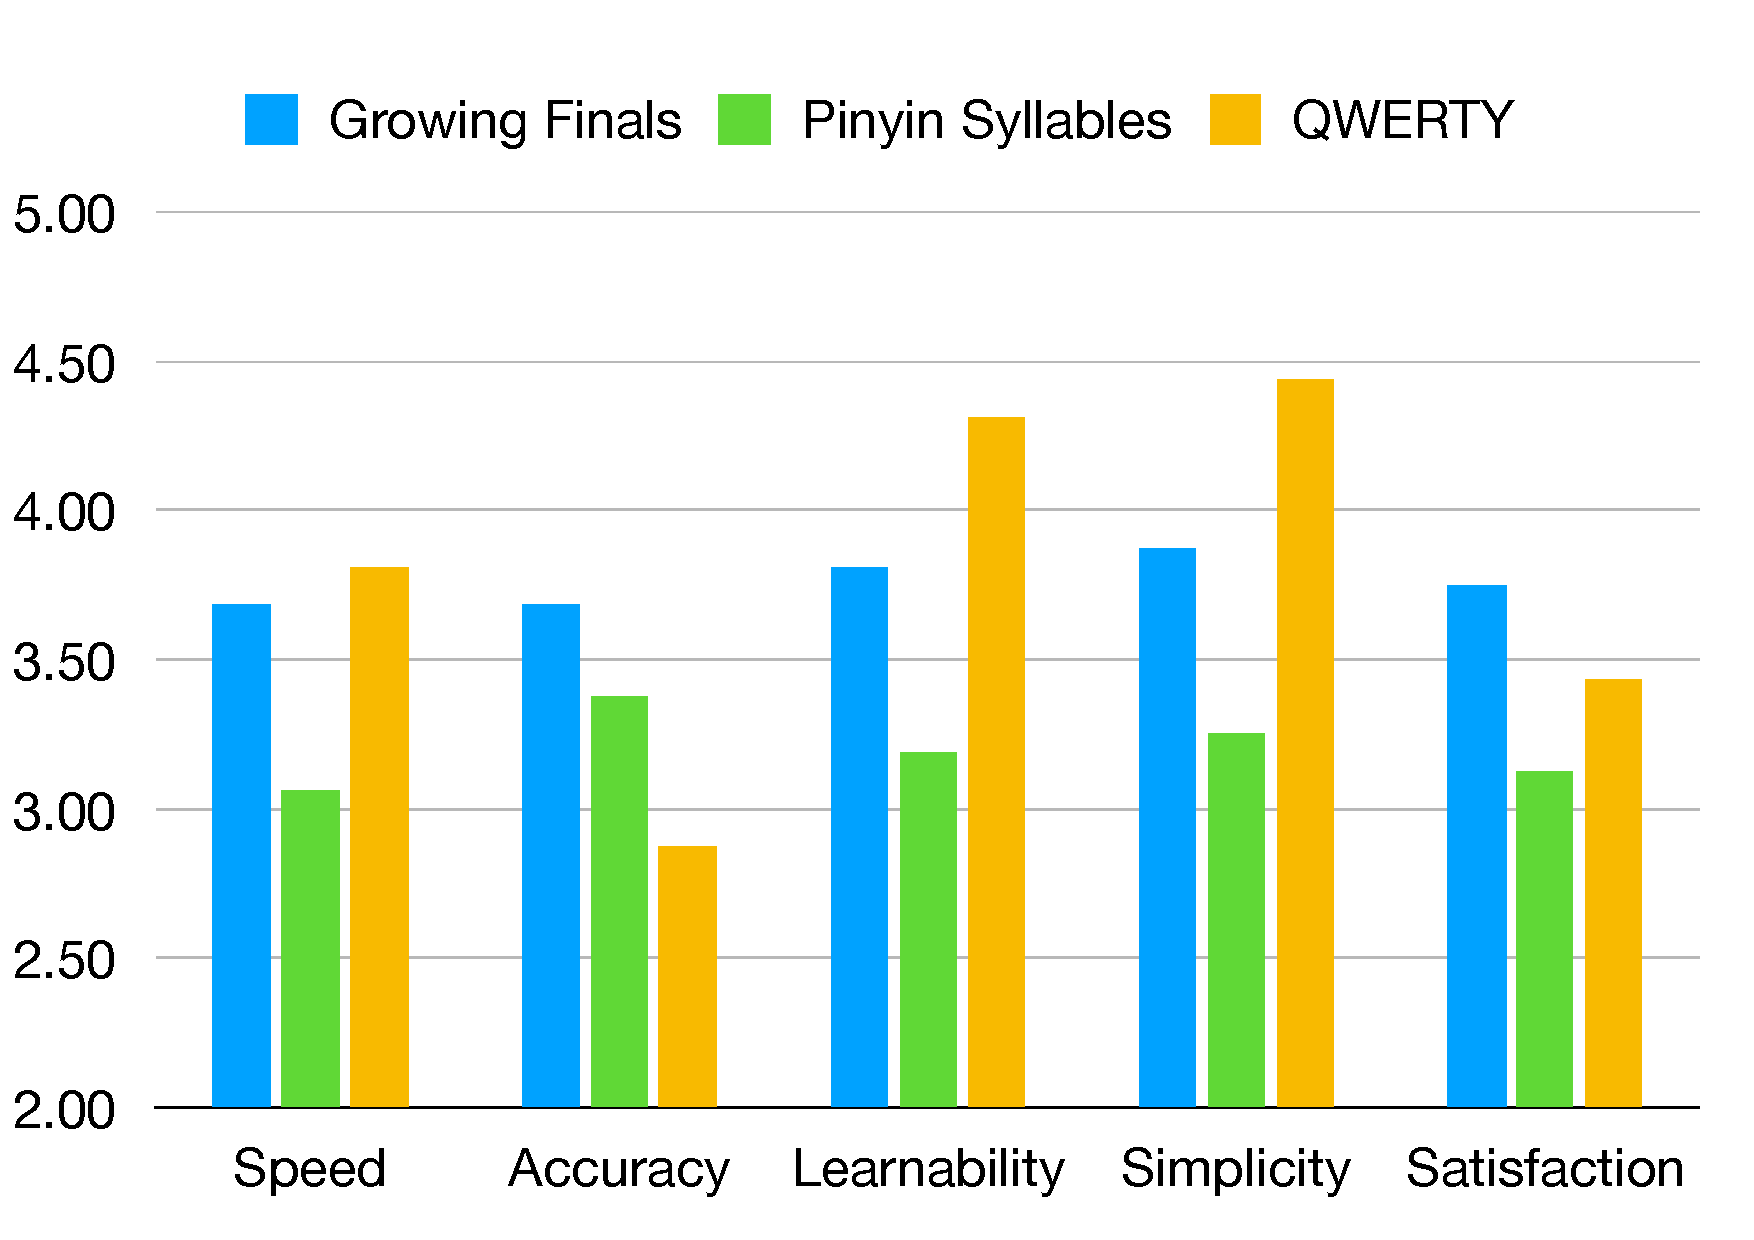
\includegraphics[width=1\columnwidth]{figures/user_prefs}
  \caption{Subjective user feedback for each keyboard prototype on a 5-point Likert scale.}~\label{fig:figure5}
\end{figure}

 
 

\section{Utilized Bandwidth}
As suggested by Soukoreff, et al. \cite{Soukoreff:2003:MTE:642611.642632} we calculate the Utilized Bandwidth (UBW) as a measure of what percentage of input events lead up to the final transcribed text and what percentage of input events are wasted on errors and correcting errors:

\[ UBW = \frac{K + S}{K + S + E + D \times 2} \]

where \textit{D} refers to the number of delete events. \textit{D} is counted twice because every delete event will undo a previously performed key event. The UBW is 100\% if no errors are made and the delete key is never used. The high UBW of 87\% (\textit{SD} = 12) of Growing Finals indicates that the delete key was necessary less often compared to other keyboard prototypes.





\section{User Preference}
Figure \ref{fig:figure5} shows the subjective user feedback. Growing Finals and QWERTY lead in terms of perceived input speed and Growing Finals and Pinyin Syllables lead in terms of typing accuracy. Overall, users were most satisfied with the Growing Finals input method.
Based on the interviews following our study, we found that more than half of our participants preferred either Growing Finals or Pinyin Syllables (Figure \ref{fig:figure6}) despite slightly lower input performance overall. Most participants where more comfortable with Growing Finals because it is similar to the familiar QWERTY layout, however some participants pointed out that Pinyin Syllables might work better for them given more time to practice and become more familiar with all the adaptive layout states.



\begin{figure}
  \centering
  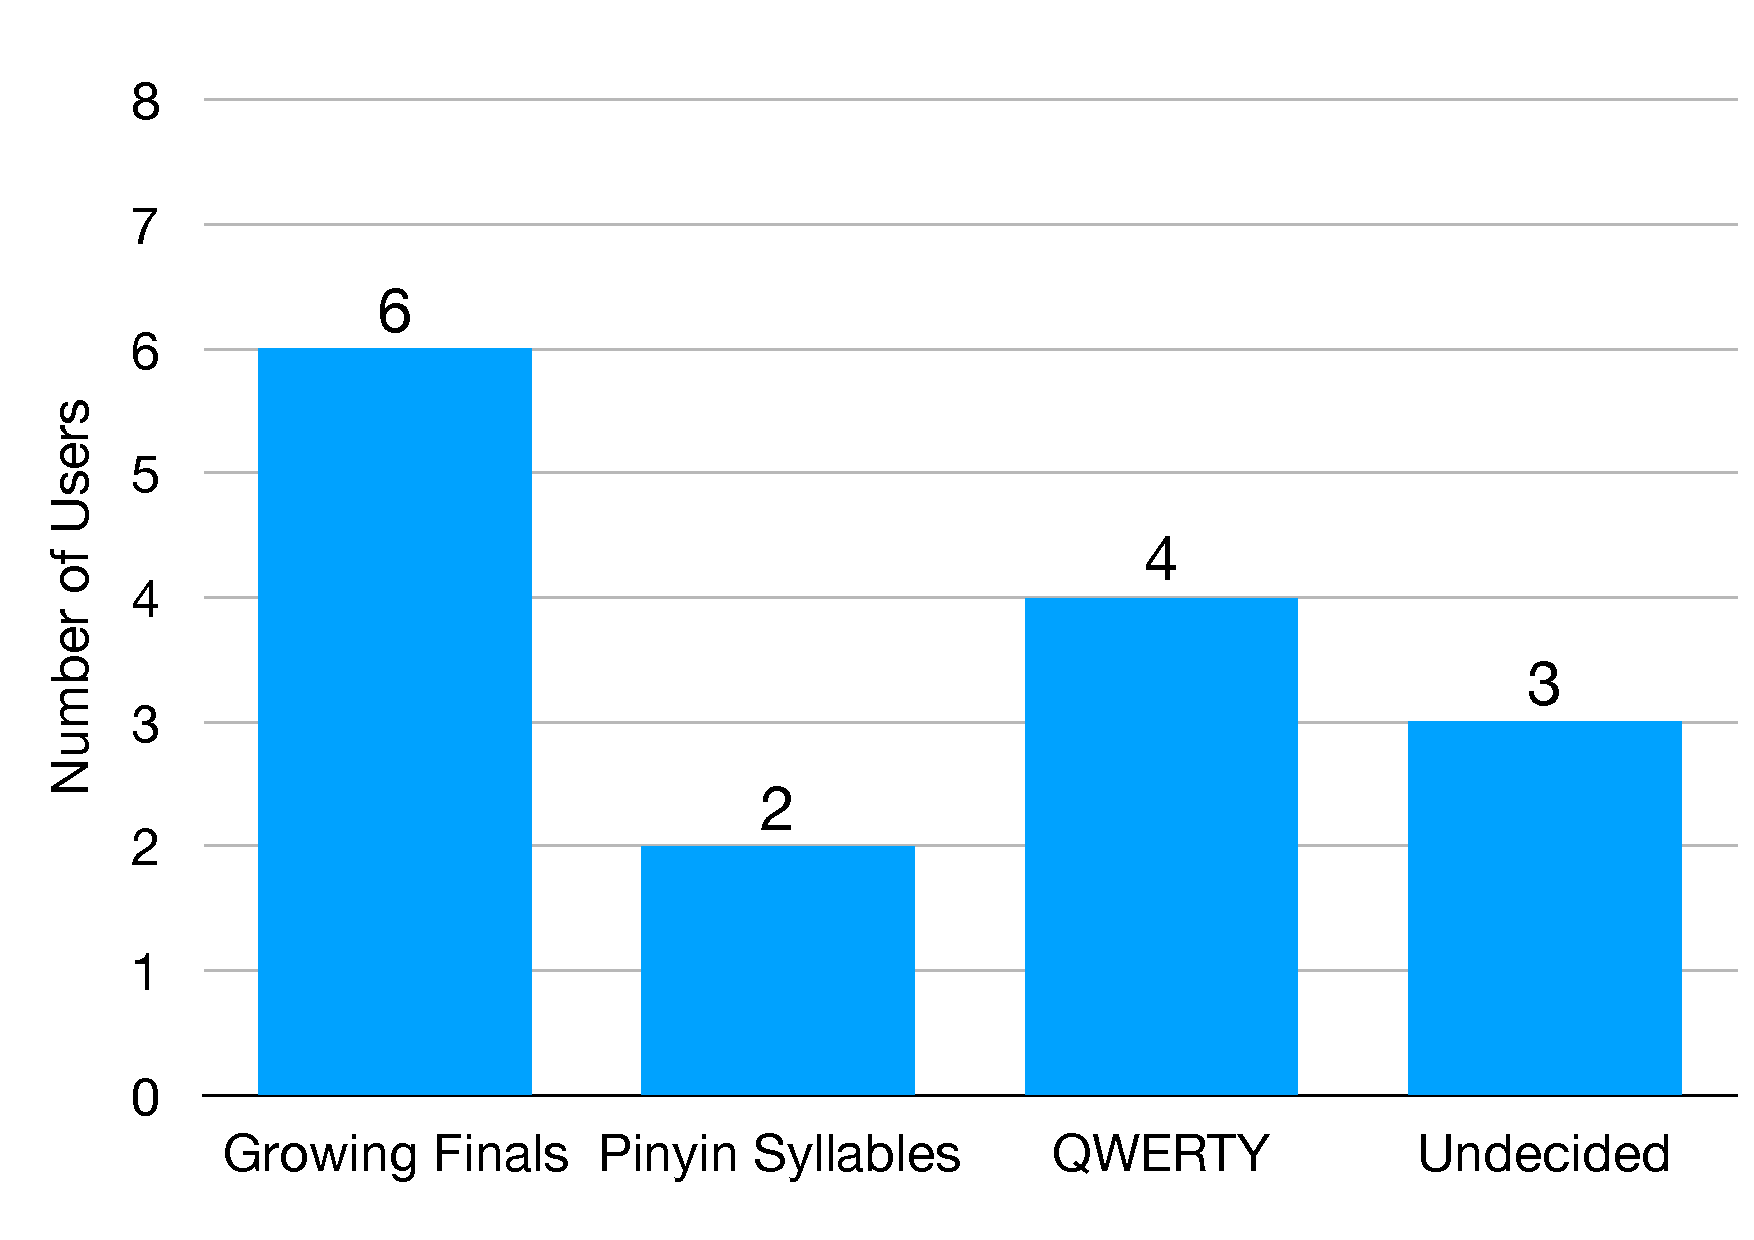
\includegraphics[width=1\columnwidth]{figures/ime_prefs}
  \caption{Preferred keyboard prototype by number of users.}~\label{fig:figure6}
\end{figure}




\chapter{Limitation and Future Work}
\label{c:limitation and future work}


There are several limitations in both implementation and evaluation of our keyboard prototypes.

Firstly, we used a single device with a 1.2" screen for the entire study. The results may vary on smaller devices. More research is needed on how these techniques fare on different smartwatches of various form factors.

Secondly, each participant was only able to use each keyboard for about 20 minutes which puts unfamiliar input methods such as Pinyin Syllables at a distinct disadvantage. In addition, some of our participants were non-native speakers and it turns out that they had trouble memorizing and transcribing each sentence correctly due to the increased cognitive load of using an unfamiliar keyboard.


\chapter{Conclusion}
\label{c:conclusion}


In this paper, we compare three keyboard layouts for Chinese text entry on smartwatches. We implement a standard QWERTY keyboard and use it as a baseline to evaluate two novel adaptive keyboard layouts specifically designed for smartwatches that use unique features of the Chinese language model and Pinyin romanization system to allow for larger keys or keys that are mapped to multiple Latin letters reducing errors and number of keystrokes required to enter a given Chinese character.

The results of our user study show that 8 out of 15 participants prefer one of our novel input methods to the standard QWERTY keyboard despite QWERTY performing slightly better in terms of Chinese characters per minute (CCPM) due to the familiarity of the keyboard layout.


\appendix

\backmatter

\addcontentsline{toc}{chapter}{\bibname}
\bibliographystyle{abbrv}

% Your bibliography goes here
\bibliography{reference_}

\end{document}
